%%%%%%%%%%%%%%%%%%%%%%%%%%%%%%%%%%%%%%%%%
% AYAB-Shield
% Soldering Manual - English
% Version 0.1 (17.11.2015)
%
% http://www.ayab-knitting.com
%
% Original authors:
% Andreas Mueller (andreas.mueller@thinkstack.de)
%
% License:
% CC BY-SA 4.0 (http://creativecommons.org/licenses/by-sa/4.0/)
%
% LaTeX Template
%
% This template has been downloaded from:
% http://www.LaTeXTemplates.com
%
% Original author:
% Mathias Legrand (legrand.mathias@gmail.com)
%
% License:
% CC BY-NC-SA 3.0 (http://creativecommons.org/licenses/by-nc-sa/3.0/)
%
%%%%%%%%%%%%%%%%%%%%%%%%%%%%%%%%%%%%%%%%%

%----------------------------------------------------------------------------------------
%   PACKAGES AND OTHER DOCUMENT CONFIGURATIONS
%----------------------------------------------------------------------------------------

\documentclass[fleqn,10pt]{SelfArx} % Document font size and equations flushed left
%\documentclass{article}
%\usepackage{lipsum} % Required to insert dummy text. To be removed otherwise

%----------------------------------------------------------------------------------------
%   COLUMNS
%----------------------------------------------------------------------------------------

\setlength{\columnsep}{0.55cm} % Distance between the two columns of text
\setlength{\fboxrule}{0.75pt} % Width of the border around the abstract

%----------------------------------------------------------------------------------------
%   COLORS
%----------------------------------------------------------------------------------------

\definecolor{color1}{RGB}{0,0,90} % Color of the article title and sections
\definecolor{color2}{RGB}{0,20,20} % Color of the boxes behind the abstract and headings

%----------------------------------------------------------------------------------------
%   Packages
%----------------------------------------------------------------------------------------
\usepackage{textgreek} % Required for Omega
\usepackage{placeins} % Required for FloatBarrier
\usepackage{wasysym} % fuer die benutzten Symbole
\usepackage{hyperref} % Required for hyperlinks
\hypersetup{hidelinks,colorlinks,breaklinks=true,urlcolor=color2,citecolor=color1,linkcolor=color1,bookmarksopen=false,pdftitle={Title},pdfauthor={Author}}

\graphicspath{ {./images/} }
%----------------------------------------------------------------------------------------
%   ARTICLE INFORMATION
%----------------------------------------------------------------------------------------

\JournalInfo{AYAB-Shield Soldering Instructions, v0.1, 2015-11-15} % Journal information
\Archive{CC BY-SA 4.0} % Additional notes (e.g. copyright, DOI, review/research article)

\PaperTitle{AYAB-Shield Soldering Instructions} % Article title

\Authors{ayab-knitting.com} % Authors
%\affiliation{\textsuperscript{1}\textit{Department of Biology, University of Examples, London, United Kingdom}} % Author affiliation
%\affiliation{\textsuperscript{2}\textit{Department of Chemistry, University of Examples, London, United Kingdom}} % Author affiliation
%\affiliation{*\textbf{Corresponding author}: john@smith.com} % Corresponding author

\Keywords{} % Keywords - if you don't want any simply remove all the text between the curly brackets
\newcommand{\keywordname}{Keywords} % Defines the keywords heading name

%----------------------------------------------------------------------------------------
%   ABSTRACT
%----------------------------------------------------------------------------------------

\Abstract{

Damages which were caused by not following the operation manual are not covered by any warranty.
For consequential damages, we do not accept liability.

}

%----------------------------------------------------------------------------------------

\begin{document}

\flushbottom % Makes all text pages the same height

\maketitle % Print the title and abstract box

\tableofcontents % Print the contents section

\thispagestyle{empty} % Removes page numbering from the first page

%----------------------------------------------------------------------------------------
%   ARTICLE CONTENTS
%----------------------------------------------------------------------------------------

%\section*{Note} % The \section*{} command stops section numbering

%\addcontentsline{toc}{section}{Introduction} % Adds this section to the table of contents

%Derjenige, der einen Bausatz fertigstellt oder eine Baugruppe durch Erweiterung bzw. Gehäuseeinbau betriebsbereit macht, gilt nach DIN VDE 0869 als Hersteller und ist verpflichtet, bei der Weitergabe des Gerätes alle Begleitpapiere mitzuliefern und auch seinen Namen und Anschrift anzugeben. Geräte, die aus Bausätzen selbst zusammengestellt werden, sind sicherheitstechnisch wie ein industrielles Produkt zu betrachten.

%------------------------------------------------

\section{Operating conditions}

\begin{itemize}[noitemsep] % [noitemsep] removes whitespace between the items for a compact look
\item This kit is not intended for usage in life-sustaining or life-saving systems or similar applications! Do not use this kit in applications, where a malfunction may lead to physical damage!
\item The kit may only be put into operation when safely built into an enclosure and safe from being touched.
\item This kit is suitable for operation in dry and clean environment only. The usage in vicinity to flammable items, water or high humidity is dangerous and prohibited.
\item This kit must not be used with or in vicinity of flammable liquids.
\item Do not exceed the electrical ratings given in this manual.
\item Assembling and operating this kit in schools or other educational environments requires supervision by skilled personnel.
\item This kit is not a toy and may be dangerous for small children! (Small parts, electrical dangers)
\item Modules and parts have to be kept away from children!
\item The kit shall only be assemblied under supervision of a skilled adult.
%\item In gewerblichen Einrichtungen sind die Vorschriften zur Unfallverhütung des Verbandes der gewerblichen Berufsgenossenschaften für elektrische Anlagen und Betriebsmittel zu beachten.
\item A repair of the device shall only be conducted by an expert!
\item If there is any liquid spilled over or into the device, it may be damaged. In this case, the device has to be checked by an expert.

\end{itemize}

%------------------------------------------------

\section{Intended Use}

The intended use of this kit is the control of Brother knitting machines, KH-9xx series.
It is only allowed to be used as a substitute for the original mainboard. An operation in parallel to the existing mainboard is not supported.

Any other usage than described above is prohibited!

%------------------------------------------------

\section{Safety Notes}

When working with products which are powered by electrical energy, you shall follow the electrical safety regulations which are  applicable for your country.
\begin{itemize}[noitemsep] % [noitemsep] removes whitespace between the items for a compact look
\item Before opening a device, always disconnect the mains connector or make sure it is disconnected.
\item Electrical parts, modules or devices shall be properly encased before being brought into operation. The case/enclosure shall prevent electrical parts from being touched.
\item Before using tools on parts, modules or devices, it has to be made sure that the power supply is disconnected and any energy storing parts are discharged.
\item Energized cables or wires which are connected to a part or module, always have to be checked for isolation faults or any other damages. If there is an isolation fault or any other damage, the device has to be taken out of service immmediately.
\item When using electrical parts or modules, the electrical and mechanical key figures shall always be regarded!
\item If electrical data does not come out clear from the manual, please contact an expert!
\item Before using a device, it shall be checked, whether this device is applicable to be used for intended application. If not sure, please contact the manufacturer or an expert!
\item Please note that usage and connection errors are out of our reach. \par Therefore, we cannot take liability for any damaged caused by such.
\item In case of a malfunction, kits shall be sent back with a detailed description of the failure. Kits which have been been built up are excluded from return.
\item Devices which operate with a voltage above 24 V have to be connected by an expert.
\item It is only allowed to switch on a device, when it is properly encased and electrical parts cannot be touched during operation.
\item All wiring work shall only be carried out in non energized state of the machine.

\end{itemize}

%------------------------------------------------

\section{Product Description}

The goal of the AYAB project is to provide an alternative way to control the famous Brother KH-9xx range of knitting machines, e.g. KH-910 and KH-930.

Normally, the KH-910 is programmed using semi-transparent picture cards which are scanned by the machine line by line. Using this information, the machine sets the needles accordingly to achieve the knitting of the picture shown on the picture card.
Probably due to memory restrictions (the machines are quite old today), the machine only supports pictures with a max of 60 needles (= pixels) width, although the machine has a total width of 200 needles. But at least, it is possible to “copy and paste” the scanned image multiple times to achieve a banner-like usage of the scanned data (useful for Norwegian patterns).

The control of the needles and the needed identification of the current position and direction of movement of the knitting carriage are supplied by a cheap and well-known Arduino microcontroller, combined with a custom developed shield (the name for an “interface” in the Arduino world) for the knitting machine.
You actually only need to open up one part of your knitting machine (warranty is void anyway for some years now…) and simply replace the existing control board (the one with all the switches and LEDs on it) with the AYAB controller, then link the Arduino part of this interface (shield) with your computer and start knitting!

The installation of AYAB is fully reversible. By installing the original control board again, the knitting machine is back in original state.

The Arduino has to be flashed with the current version of the AYAB firmware. A precompiled version of the firmware is shipped with the AYAB GUI and is also available [here] (choose the right Arduino type). For flashing instructions, check the tutorial video.

The AYAB project is free and open source soft- and hardware. Source code and schematics are available freely available and free for customization. Of course, we are always happy about feedback and participation in the project!

 \subsection*{Properties}

Supported Models: Brother KH-910, Brother KH-930 (further models will be officially added soon)
Maximum Pattern Width: 200 Needles
Maximum Pattern Length: unlimited
Maximum Colors: 2 (up to 6 experimental)

 \subsection*{Note}

Please take care to chose the right machine model when ordering a shield to make sure the right connectors are shipped.

%------------------------------------------------

\section{Technical Data}

\begin{tabular}{ll}
Supply Voltage            & 5.0 V              \\ \hline
Switching Voltage         & 7.5V - 16.0V       \\ \hline
max. Current Consumption  & 500 mA             \\ \hline
max. Switching Current    & 1500 mA            \\ \hline
Dimensions (l x w x h)    & 69 mm x 54 mm x 20 mm
\end{tabular}


%------------------------------------------------

\section{Before you start}

Before you start with the installation, please read this manual completely - especially the section about error sources and the safety notes. After this, you will know about common problems and how to avoid errors which can only be solved with high effort!

Please do soldering and wiring work clean and precisely. Do not use acidic solder or soldering flux. Please make sure that all solder joints are working correctly. Unclean or bad solder joints and loose contacts may lead to an elaborate and time-consuming fault analysis. It may also lead to the destruction of parts, which may also harm other modules or even the knitting machine.

For assembling this kit, basic knowledge about handling of electrical parts and soldering is necessary.

 \subsection*{General Notes}

You can reduce the possibility of a malfunction drastically by doing a clean and precise assembly. Please double check each solder joint and working step before proceeding. Please stick to this manual!
90% of malfunctions are caused by erroneous soldering.

This kit was built and tested many times before going into production.

%------------------------------------------------

\section{Assembling the parts on the board}

 \subsection*{Note}

While working, please stick to this manual and always keep an eye on the assembly diagram in parallel.

Please pay attention to the polarity/orientation of the three LEDs.

Please pay attention to the marking notch of the ICs. The orienation has to match with the assembly diagram.

Double check the position and orientation of all parts before initial operation.

Please pay attention to solder all parts directly onto the board (without any air gap). All projecting pins and leads have to be cut of directly above the soldering joint.

Because there are some small soldering joints to do, this kit may only be soldered with a soldering iron with appropriate soldering tip. Please take care to avoid short-circuits.

 \subsection*{Solder instruction}

If you are not used to solder wired components, please read a solder guid for wired components. You can find such in the Internet or on our homepage.

\url{http://ayab-knitting.com}

Please note that some parts (especially the ICs) are temperature sensitive. Do not overheat them during soldering!

 \subsection*{Step 1: LEDs}


\begin{tabular}{ll}
\hline
\textbf{Name} & \textbf{Color}  \\ \hline
LED1          & red             \\ \hline
LED2          & yellow          \\ \hline
LED2          & green           \\ \hline
\end{tabular}\\

Place the three LEDs (red, yellow, green) according to the figure \ref{fig:abb1_1} on the board. Please double check the polarity and have a look at the silkscreen.

After placing the LEDs, please solder them on the bottom side of the board.

\begin{figure}[tbhp]\centering
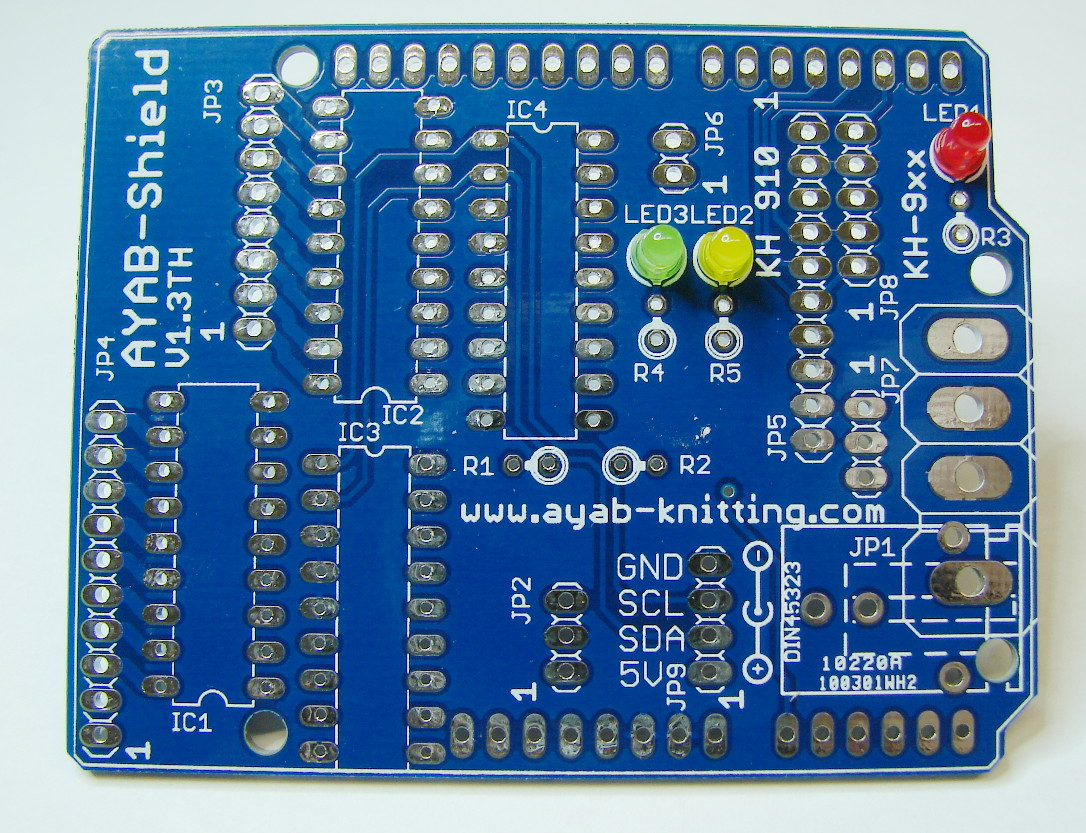
\includegraphics[width=\linewidth]{abb1_1}
\caption{LEDs}
\label{fig:abb1_1}
\end{figure}

\FloatBarrier

 \subsection*{Step 2: Resistors}

The AYAB shield kit contains to types of resistors\\

\begin{tabular}{lll}
\hline
\textbf{Name} & \textbf{Value}           & \textbf{Colors} \\ \hline
R1            & 10k\textOmega            & br-sw-or-gd \\ \hline
R2            & 10k\textOmega            & br-sw-or-gd \\ \hline
R3            & 150\textOmega            & br-gr-br-gd \\ \hline
R4            & 150\textOmega            & br-gr-br-gd \\ \hline
R5            & 150\textOmega            & br-gr-br-gd \\ \hline
\end{tabular}\\

Please bend all resistors according to figure \ref{fig:abb2_1}.

\begin{figure}[tbhp]\centering
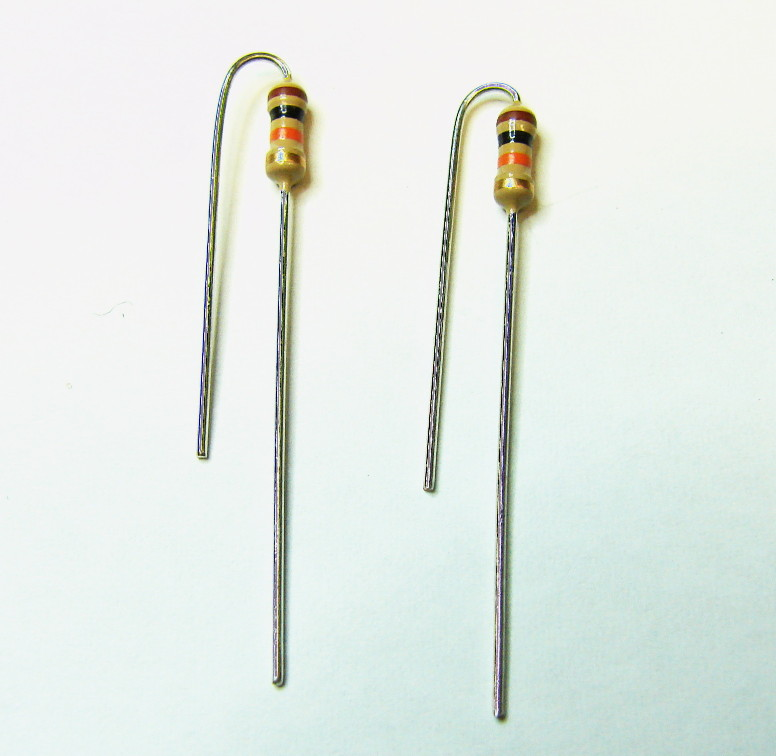
\includegraphics[width=\linewidth]{abb2_1}
\caption{Bending the resistors}
\label{fig:abb2_1}
\end{figure}

Place the 150\textOmega resistors according to figure \ref{fig:abb2_2} and solder them. Next, please place the 10k\textOmega resistors according to figure \ref{fig:abb2_3} and solder them.

\begin{figure}[tbhp]\centering
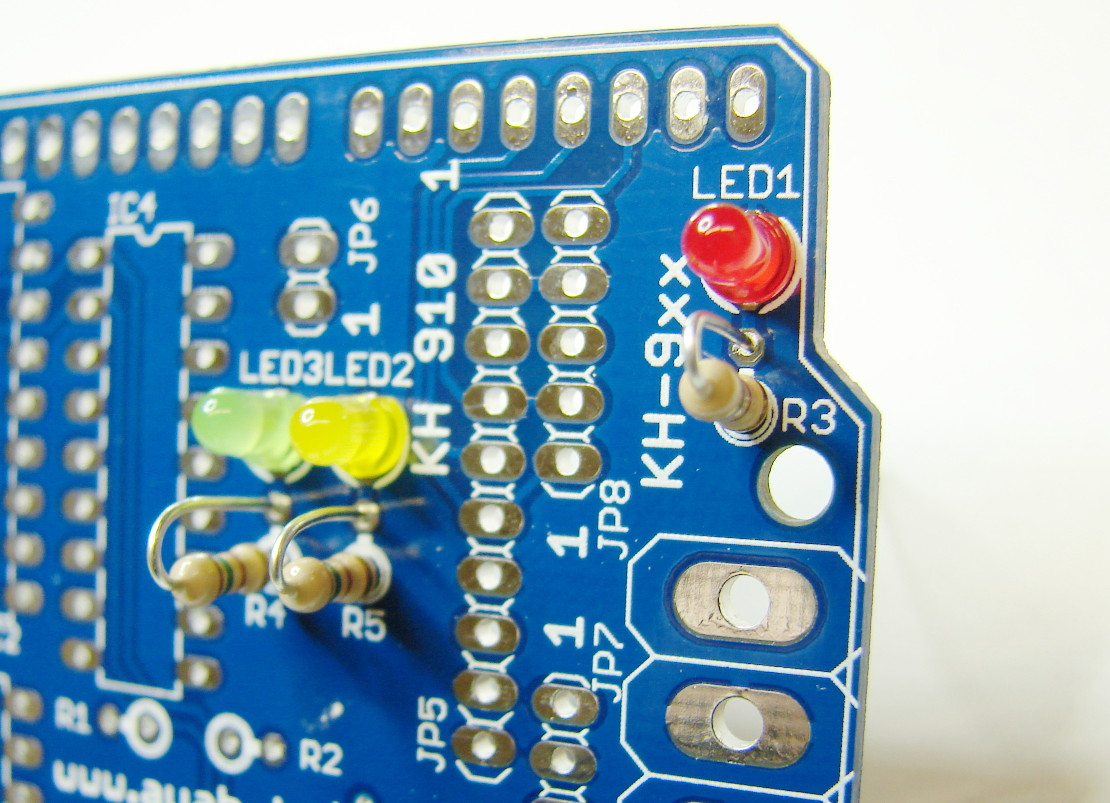
\includegraphics[width=\linewidth]{abb2_2}
\caption{150\textOmega resistors}
\label{fig:abb2_2}
\end{figure}

\begin{figure}[tbhp]\centering
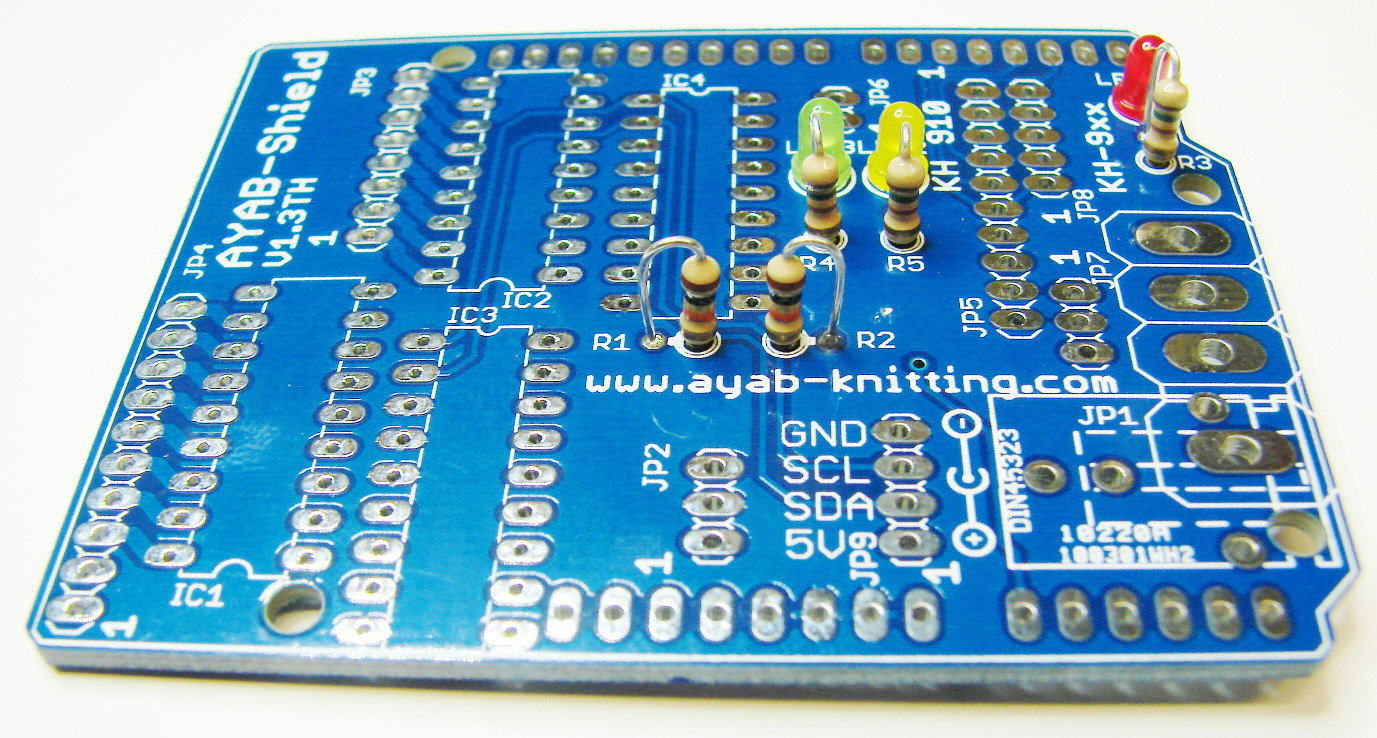
\includegraphics[width=\linewidth]{abb2_3}
\caption{10k\textOmega resistors}
\label{fig:abb2_3}
\end{figure}

\FloatBarrier

 \subsection*{Step 3: Machine connectors}

\textbf{WARNING!} This section is handled differently, based on your machine model.\\

\textbf{KH-910 / KH-950:} \\

\begin{tabular}{lll}
\hline
\textbf{Name} & \textbf{Pin count}  & \textbf{Type} \\ \hline
JP3           & 8                 & angle        \\ \hline
JP4           & 10                & angle        \\ \hline
JP5           & 10                & straight     \\ \hline
JP9           & 4                 & straight     \\ \hline
\end{tabular}\\

Please solder connectors JP3, JP4 and JP5 according to figure \ref{fig:abb3_1}. Please take care to solder JP4 with a small gap (figure \ref{fig:abb3_2}), to ease the connection with the knitting machine. You can help yourself by putting a washer below the connector while soldering.

\begin{figure}[tbhp]\centering
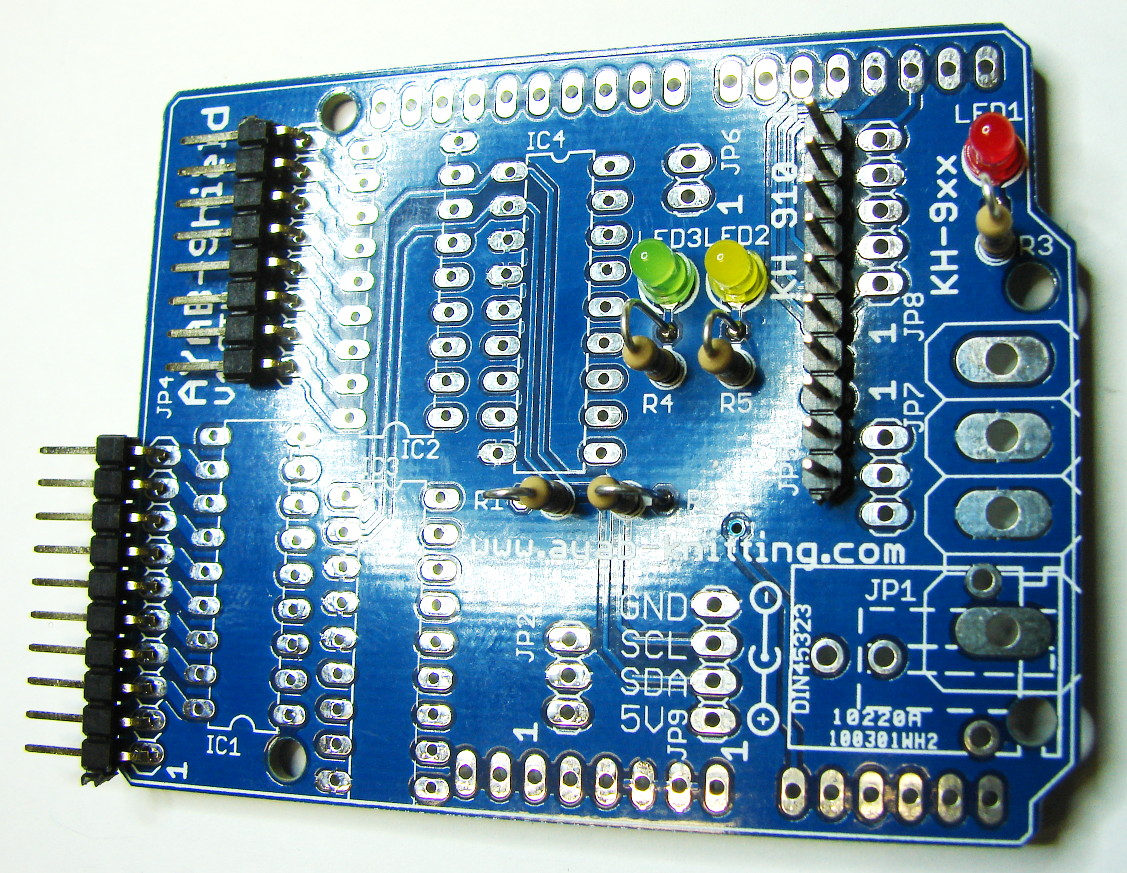
\includegraphics[width=\linewidth]{abb3_1}
\caption{Machine Connectors KH-910/KH-950}
\label{fig:abb3_1}
\end{figure}

\begin{figure}[tbhp]\centering
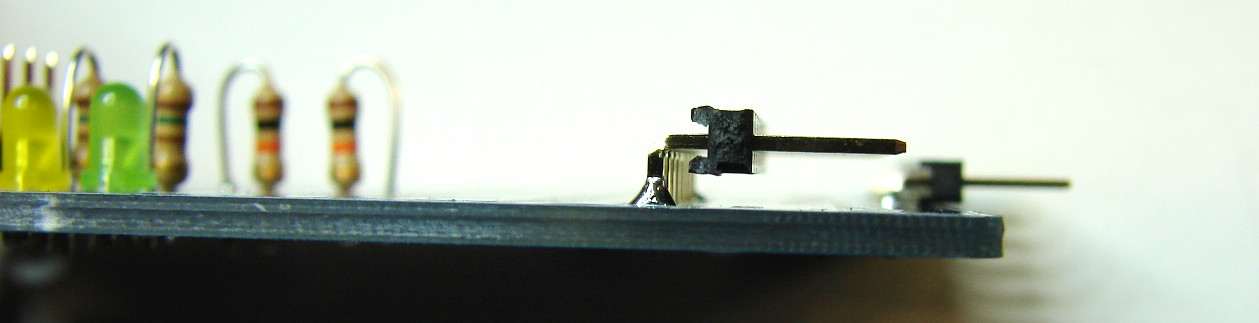
\includegraphics[width=\linewidth]{abb3_2}
\caption{Gap JP3}
\label{fig:abb3_2}
\end{figure}

Optionally, you can solder the expansion connector JP9 (figure \ref{fig:abb3_3}). In the future, this connector can be used to connect i.e. an optional color changer \par

\begin{figure}[tbhp]\centering
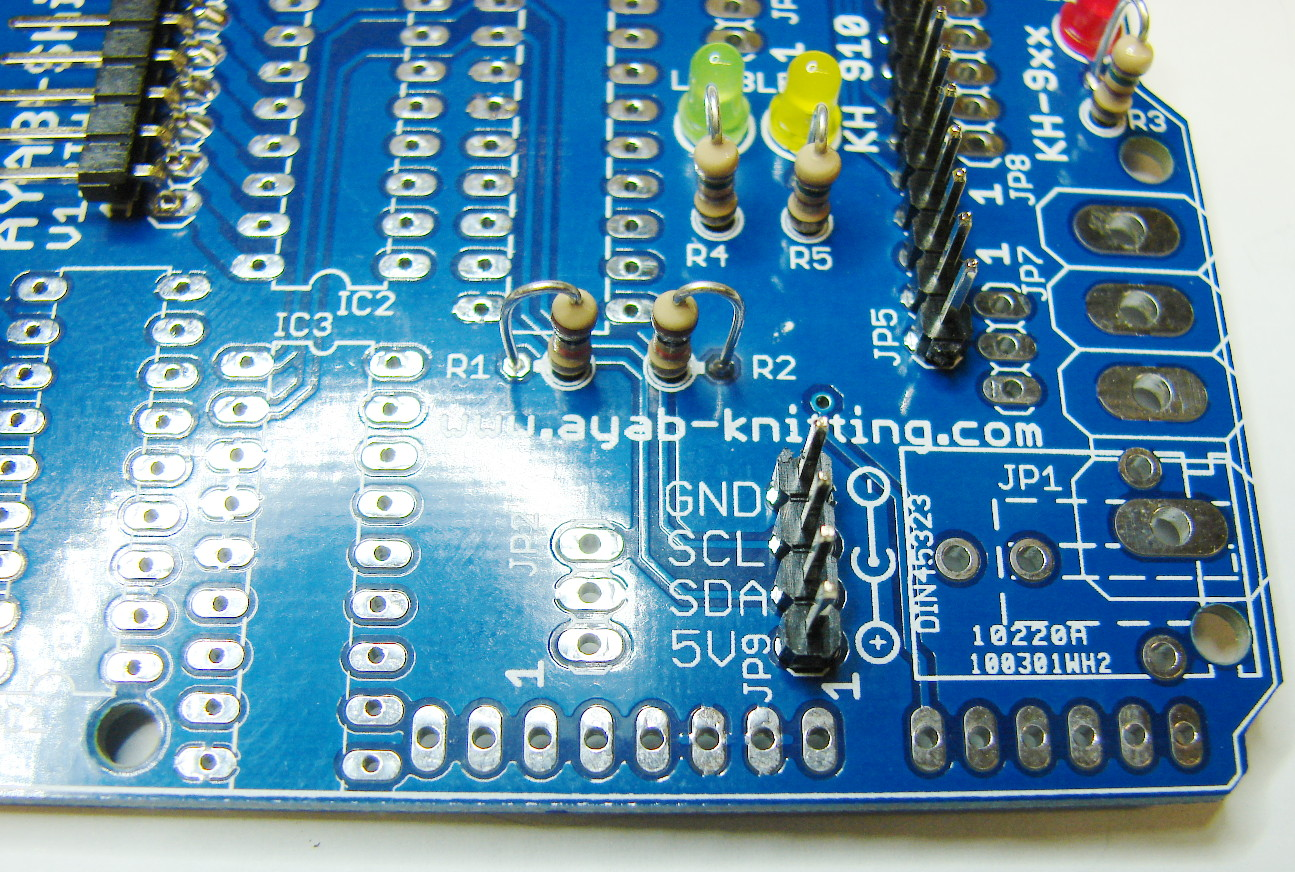
\includegraphics[width=\linewidth]{abb3_3}
\caption{Expansion connector}
\label{fig:abb3_3}
\end{figure}

\FloatBarrier

\textbf{KH-930:} \\

\begin{tabular}{lll}
\hline
\textbf{Name} & \textbf{Pin count}  & \textbf{Type} \\ \hline
JP3           & 8                 & Molex 2.5mm  \\ \hline
JP4           & 10                & Molex 2.5mm  \\ \hline
JP2           & 3                 & Molex 2.5mm  \\ \hline
JP8           & 5                 & Molex 2.5mm  \\ \hline
JP9           & 4                 & straight     \\ \hline
\end{tabular}\\

Solder the connectors JP3, JP4, JP2 and JP8 according to figure \ref{fig:abb3_4}. Please double check the correct orientation of the connectors!

\begin{figure}[tbhp]\centering
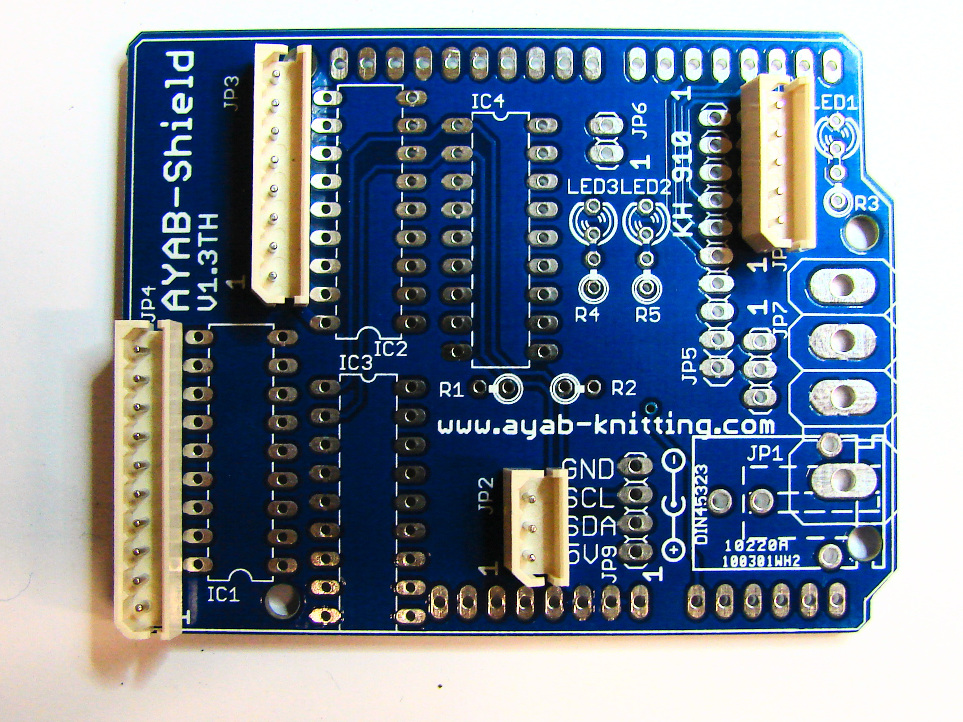
\includegraphics[width=\linewidth]{abb3_4}
\caption{Machine connectors KH-930}
\label{fig:abb3_4}
\end{figure}

Optionally, you can solder the expansion connector JP9 (figure \ref{fig:abb3_3}). In the future, this connector can be used to connect i.e. an optional color changer \par

\FloatBarrier

 \subsection*{Step 4: Beeper connector}

Now, you can solder the connector for the beeper, like shown in figure \ref{fig:abb4_1}. As before, please double check the orientation of the connector and avoid a gap between the connector and the board.

\begin{figure}[tbhp]\centering
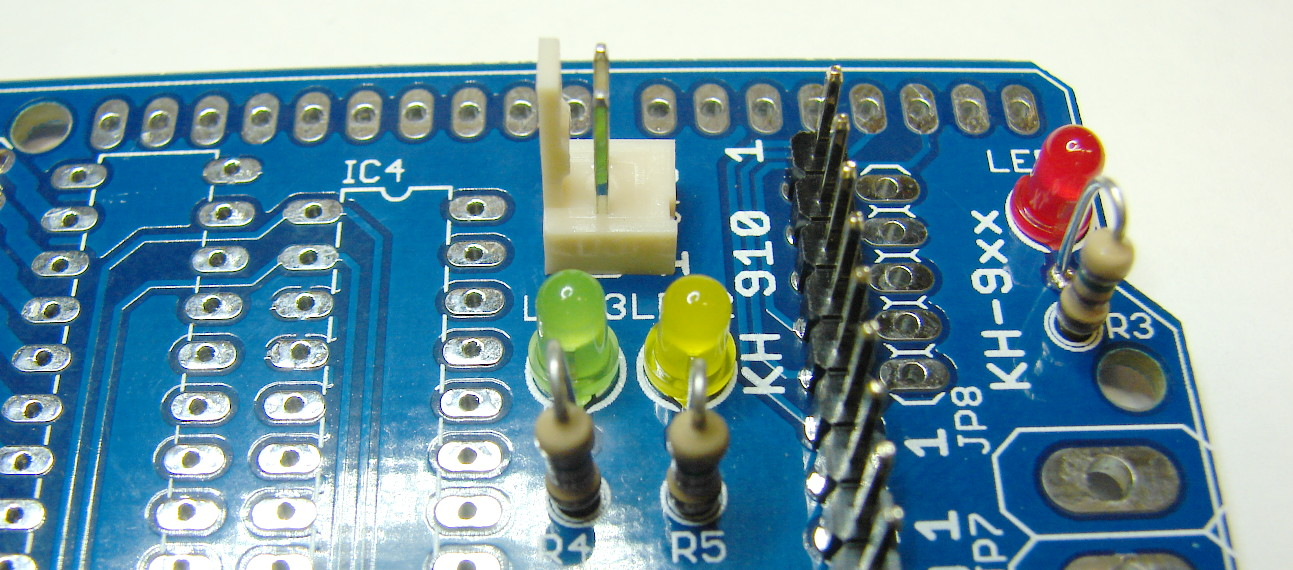
\includegraphics[width=\linewidth]{abb4_1}
\caption{Beeper connector}
\label{fig:abb4_1}
\end{figure}

\FloatBarrier

 \subsection*{Step 5: Arduino connectors}

\textbf{Arduino not included in kit}\\

The following connectors are needed:\\

\begin{tabular}{lll}
\hline
\textbf{Name} & \textbf{Pin count}  & \textbf{Type} \\ \hline
ARD1          & 10                & straight       \\ \hline
ARD2          & 8                 & straight       \\ \hline
ARD3          & 8                 & straight       \\ \hline
ARD4          & 6                 & straight       \\ \hline
\end{tabular}\\


\textbf{Tip!} Put the four connectors into the Arduino as a soldering aid (figure \ref{fig:abb5_1}) and place the shield onto (figure \ref{fig:abb5_2}). This eases the soldering work significantly and makes sure everything fits right.

\begin{figure}[tbhp]\centering
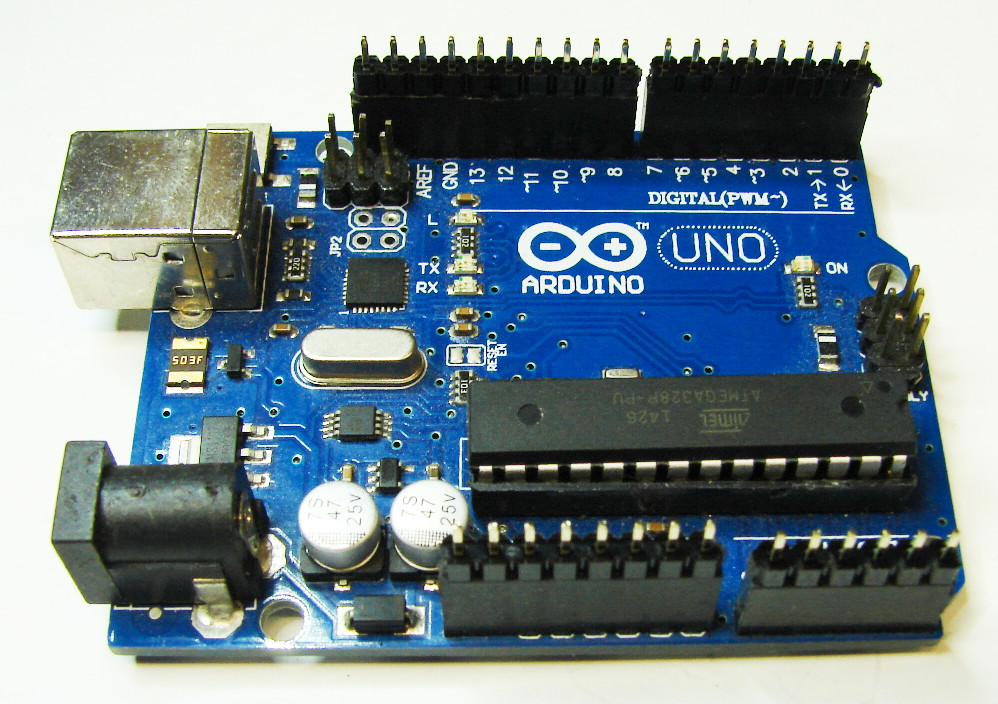
\includegraphics[width=\linewidth]{abb5_1}
\caption{Soldering aid}
\label{fig:abb5_1}
\end{figure}

\begin{figure}[tbhp]\centering
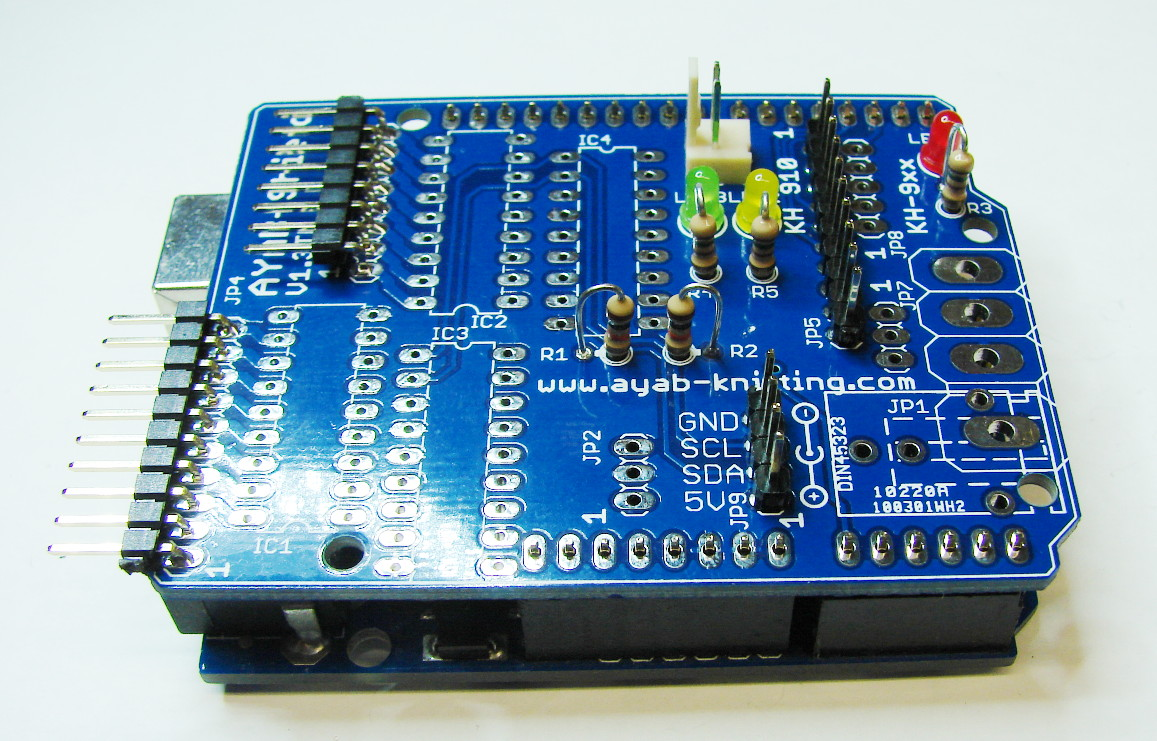
\includegraphics[width=\linewidth]{abb5_2}
\caption{Arduino connectors}
\label{fig:abb5_2}
\end{figure}

\FloatBarrier

 \subsection*{Step 6: ICs}

\textbf{WARNING!} Please double check the orientation of the ICs. The markings have to be oriented according to \ref{fig:abb6_1}. Pay attention that IC1 and IC2 have different orientation as IC3 and IC4! Be careful when inserting the ICs into the board. Do not overheat the ICs!\\
\begin{tabular}{ll}
\hline
\textbf{Name} & \textbf{Type} \\ \hline
IC1           & ULN 2803 L   \\ \hline
IC2           & ULN 2803 L   \\ \hline
IC3           & MCP 23008    \\ \hline
IC4           & MCP 23008    \\ \hline
\end{tabular}\\

\begin{figure}[tbhp]\centering
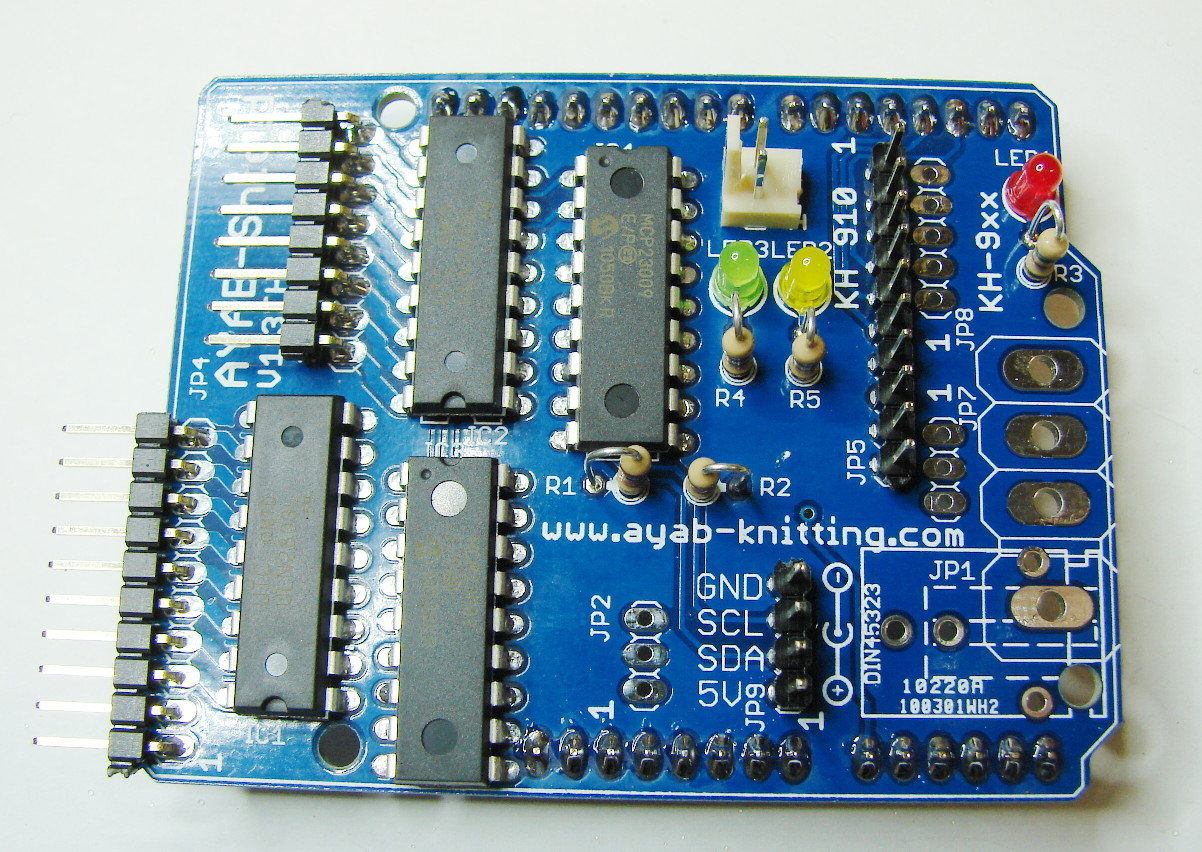
\includegraphics[width=\linewidth]{abb6_1}
\caption{ICs}
\label{fig:abb6_1}
\end{figure}

\FloatBarrier

 \subsection*{Step 7: Sensor wires}

\textbf{WARNING!} This section is handled differently, based on your machine model.\\

\textbf{KH-910 / KH-950:} \\

Strip the insulation of the ribbon cable according to figure \ref{fig:abb7_1}.

\begin{figure}[tbhp]\centering
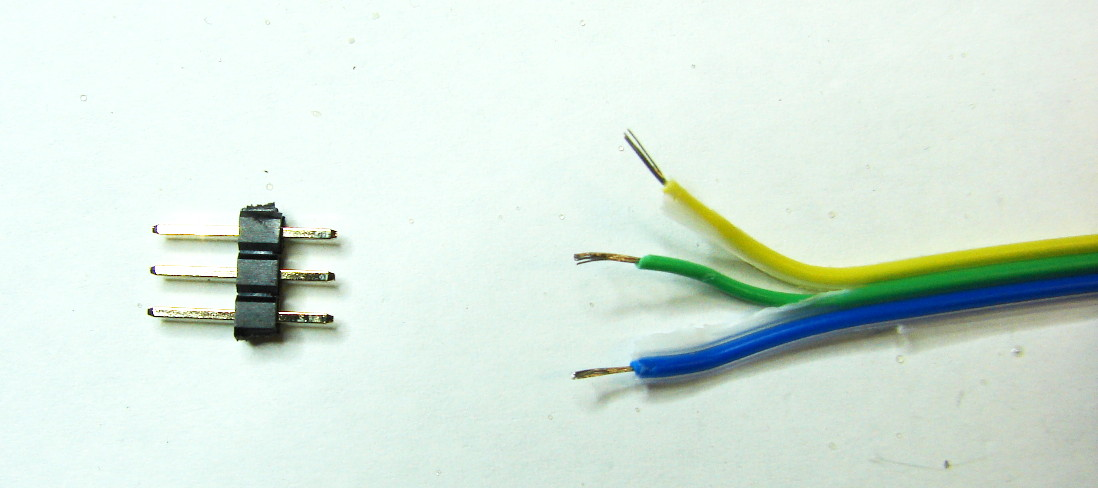
\includegraphics[width=\linewidth]{abb7_1}
\caption{Strip the insulation (KH-910/KH-950)}
\label{fig:abb7_1}
\end{figure}

Tin-coat the wire endings and the 3 pin connector (figure \ref{fig:abb7_2}) and solder them together (figure \ref{fig:abb7_3}). Double check for mechanical stability and potential short circuits. It is recommended to use shrinking tube for better stability and short circuit avoidance.

\begin{figure}[tbhp]\centering
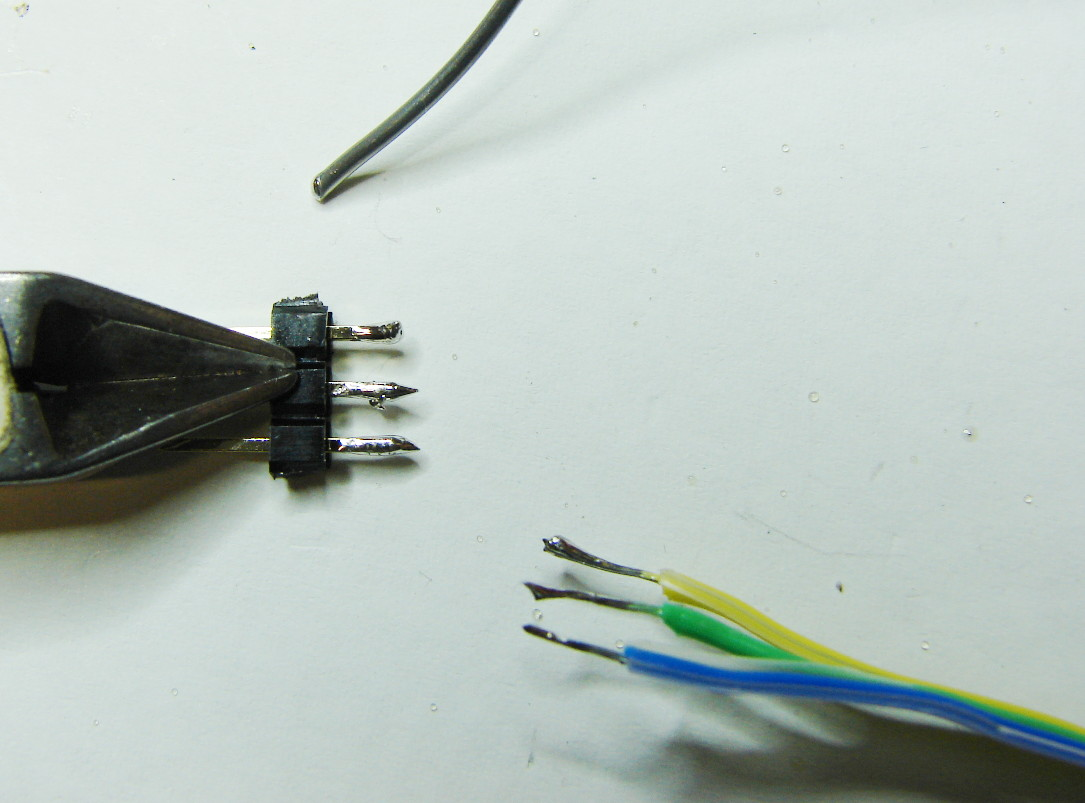
\includegraphics[width=\linewidth]{abb7_2}
\caption{Tin coating (KH-910/KH-950)}
\label{fig:abb7_2}
\end{figure}

\begin{figure}[tbhp]\centering
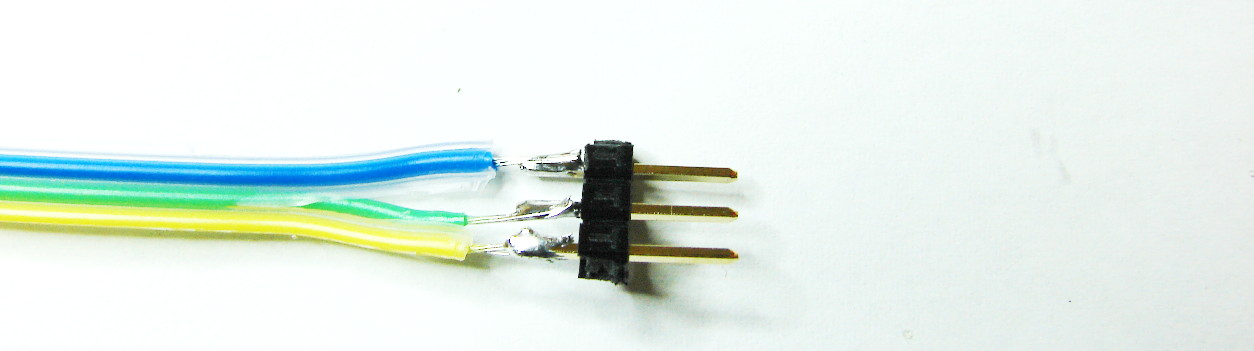
\includegraphics[width=\linewidth]{abb7_3}
\caption{Soldered wire ends (KH-910/KH-950)}
\label{fig:abb7_3}
\end{figure}

Now solder the other end of the ribbon cable like shown in figure \ref{fig:abb7_4} to JP2 and mark the top side of the connector like shown in figure \ref{fig:abb7_5}. This helps when installing the shield into the machine.\par

\begin{figure}[tbhp]\centering
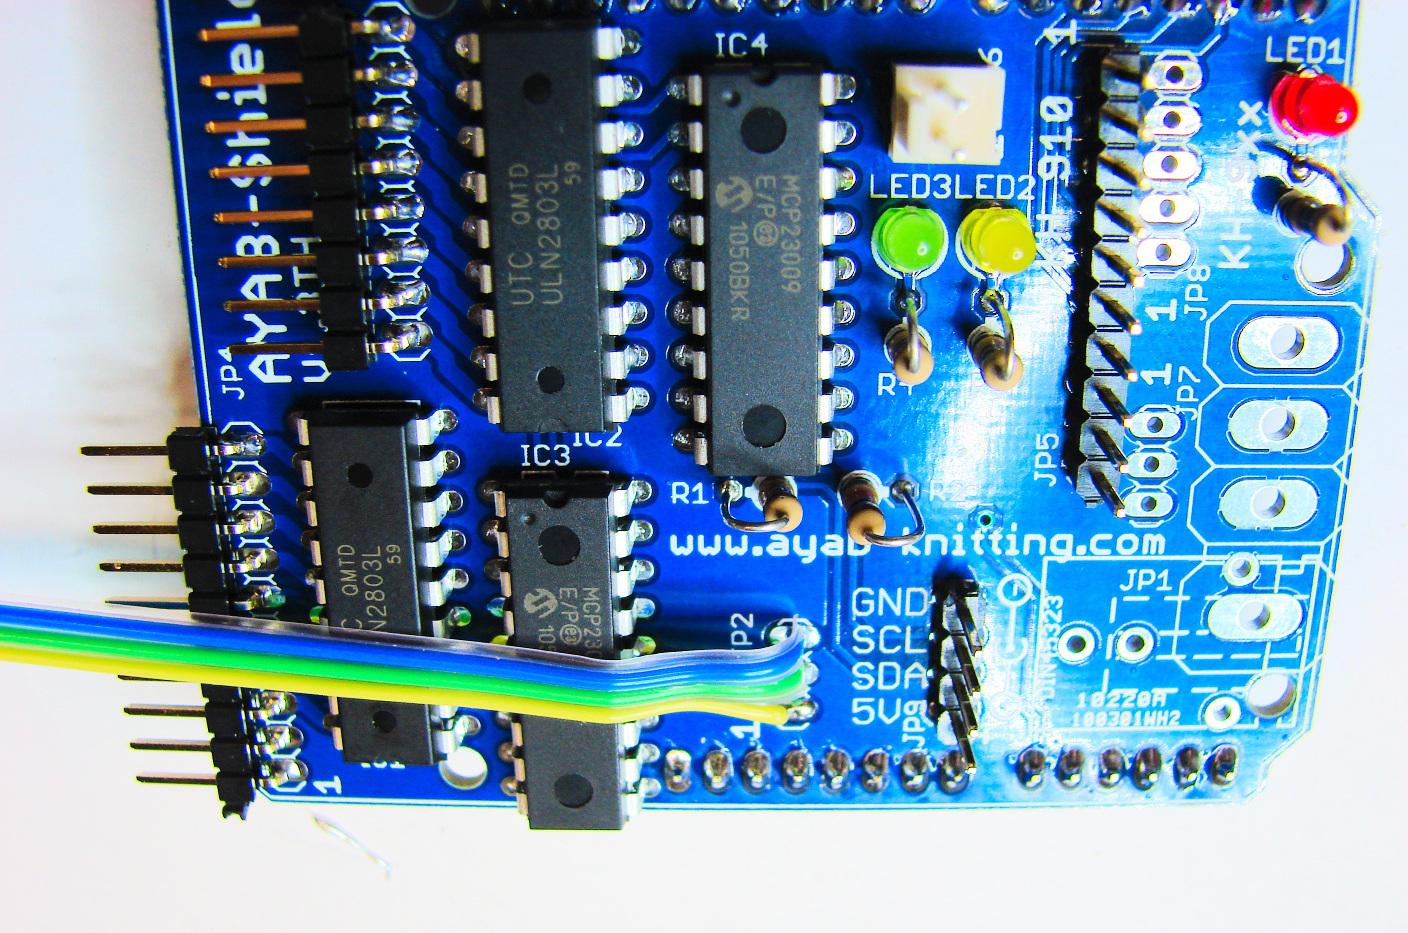
\includegraphics[width=\linewidth]{abb7_4}
\caption{Connection to board (KH-910/KH-950)}
\label{fig:abb7_4}
\end{figure}

\begin{figure}[tbhp]\centering
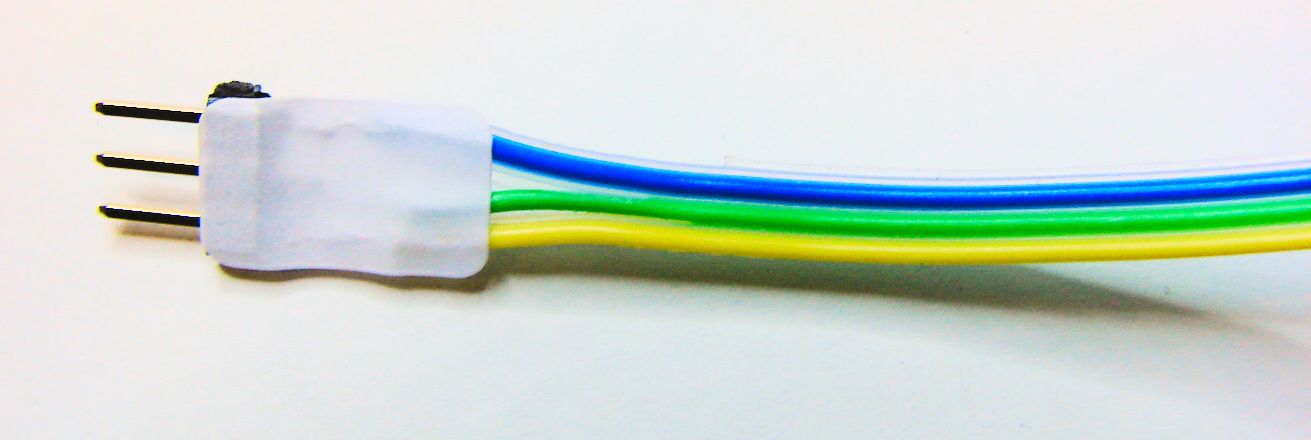
\includegraphics[width=\linewidth]{abb7_5}
\caption{Marking the connector (KH-910/KH-950)}
\label{fig:abb7_5}
\end{figure}

\FloatBarrier

\textbf{KH-930:} \\

Strip the insulation of the ribbon cable according to figure \ref{fig:abb7_6} ab.

\begin{figure}[tbhp]\centering
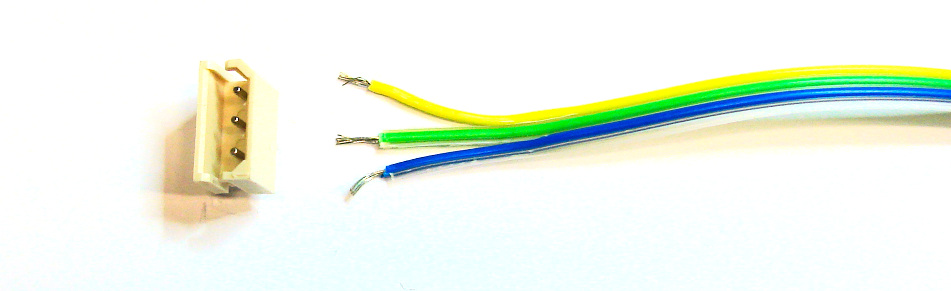
\includegraphics[width=\linewidth]{abb7_6}
\caption{Strip the insulation (KH-930)}
\label{fig:abb7_6}
\end{figure}

Tin-coat the wire endings and the 3 pin Molex connector and solder them together. Double check for mechanical stability and potential short circuits. It is recommended to use shrinking tube for better stability and short circuit avoidance.

Now solder the other end of the ribbon cable like shown in figure \ref{fig:abb7_7} to JP7. Double check the orientation of the connector. The markings of the connector have to point \textbf{to} the red LED (in contrast to the other machine connectors).

\begin{figure}[tbhp]\centering
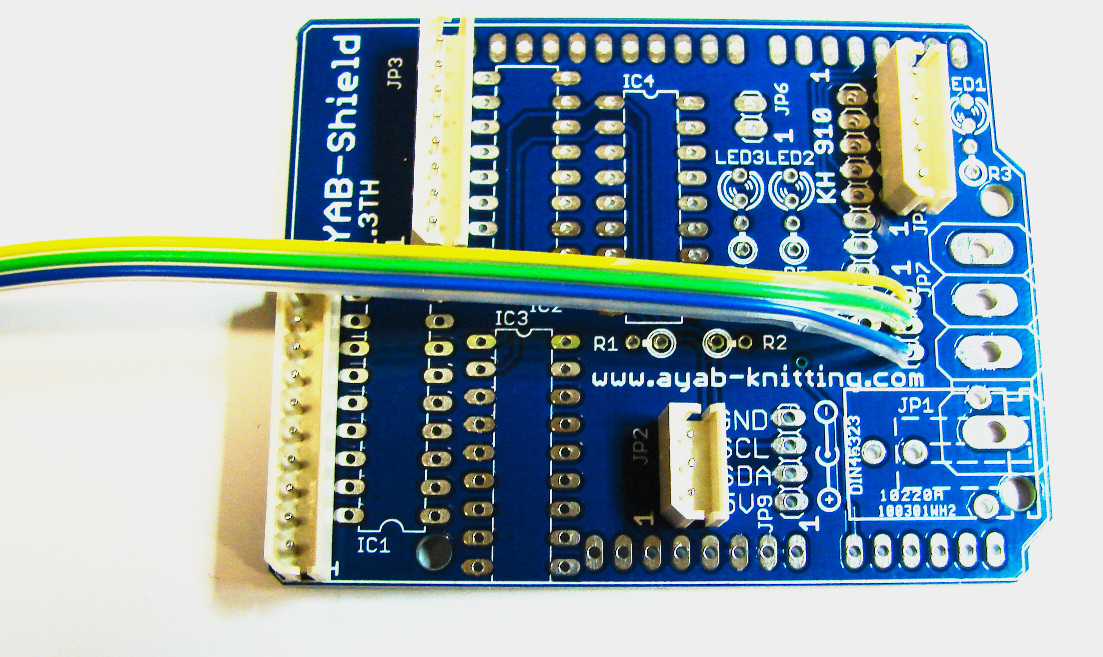
\includegraphics[width=\linewidth]{abb7_7}
\caption{Connection to board (KH-930)}
\label{fig:abb7_7}
\end{figure}

\FloatBarrier

 \subsection*{Step 8: Power connector}

\textbf{WARNING!} This section is handled differently, based on your machine model.\\

\textbf{KH-910 / KH-930 / KH-950 / CK-35:} \\

Please mount and solder the 4 pin connector according to figure \ref{fig:abb8_1}. Please take care of uniform height of all pins and correct carefully, if necessary.

\begin{figure}[tbhp]\centering
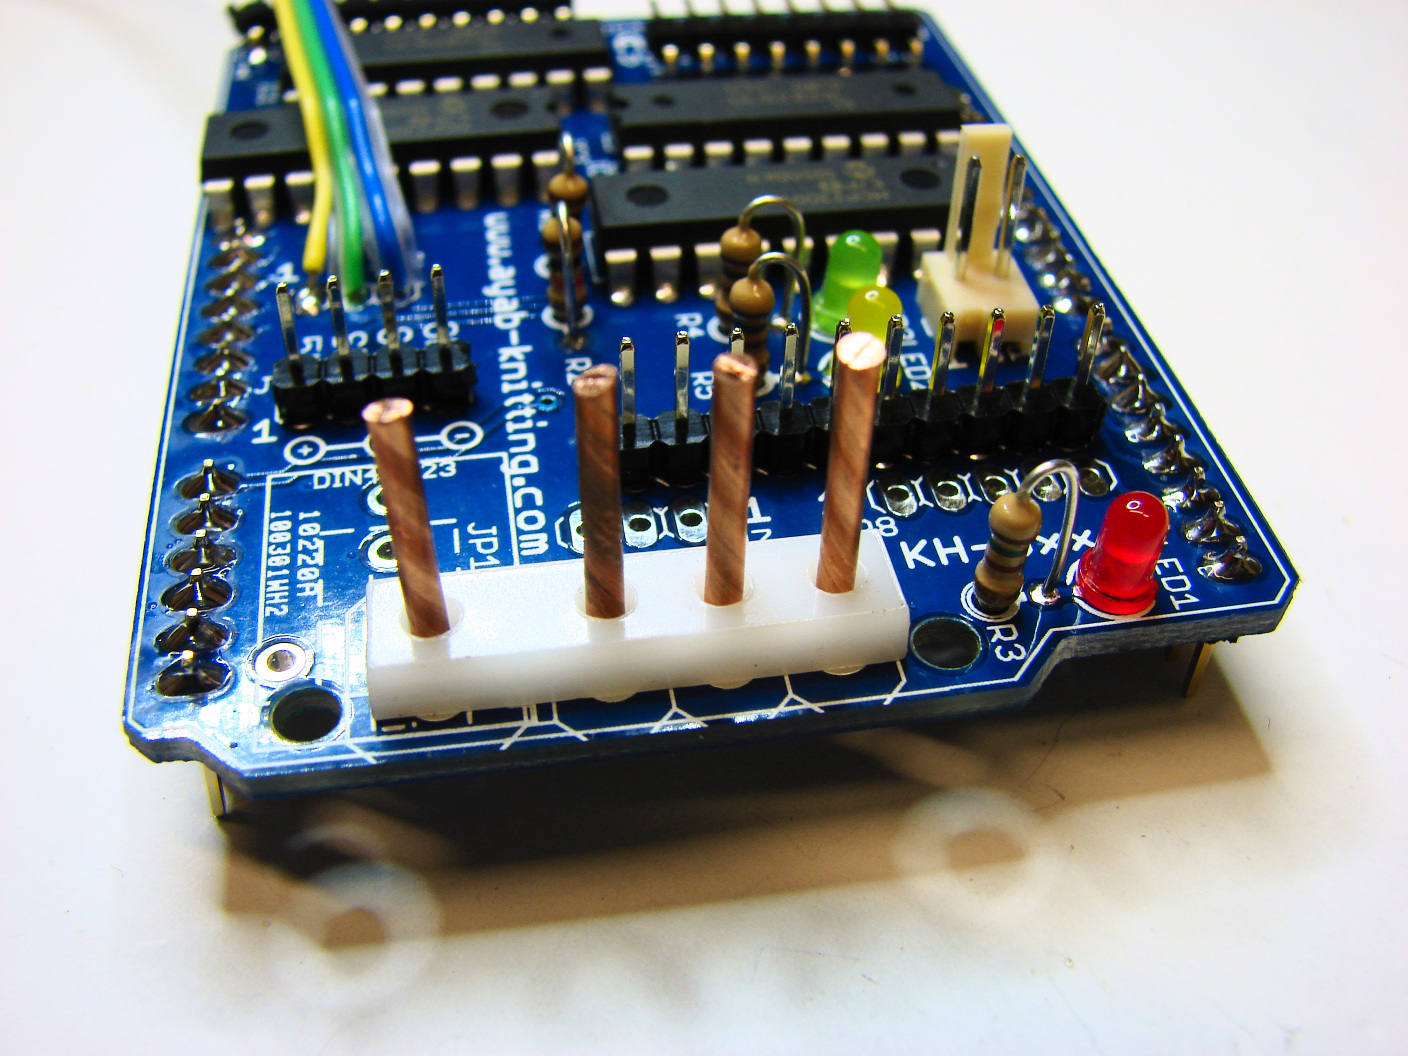
\includegraphics[width=\linewidth]{abb8_1}
\caption{Power connector KH-910/930/950 and CK35}
\label{fig:abb8_1}
\end{figure}

Now, on the bottom side of the board, the pins have to be cut of as near as possible to the board (see figures \ref{fig:abb8_2} and \ref{fig:abb8_2b}) to avoid short-circuits with the ISP pins of the Arduino. Additionally, the pins can be insulated using insulating/duct tape\par

\begin{figure}[tbhp]\centering
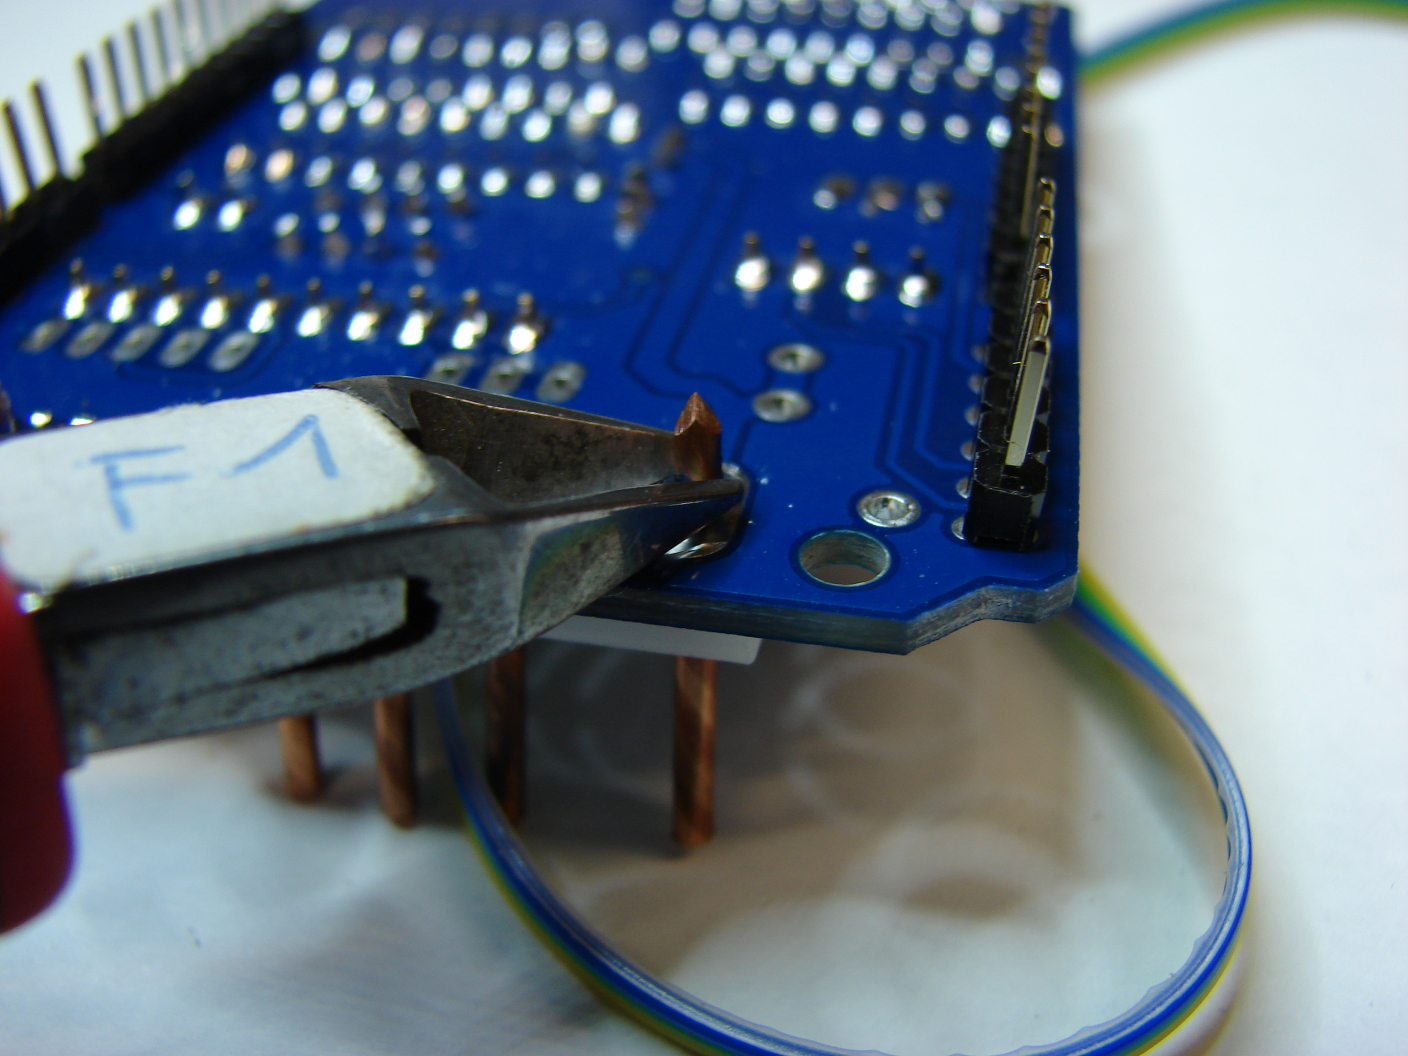
\includegraphics[width=\linewidth]{abb8_2}
\caption{Avoid short-circuits}
\label{fig:abb8_2}
\end{figure}

\begin{figure}[tbhp]\centering
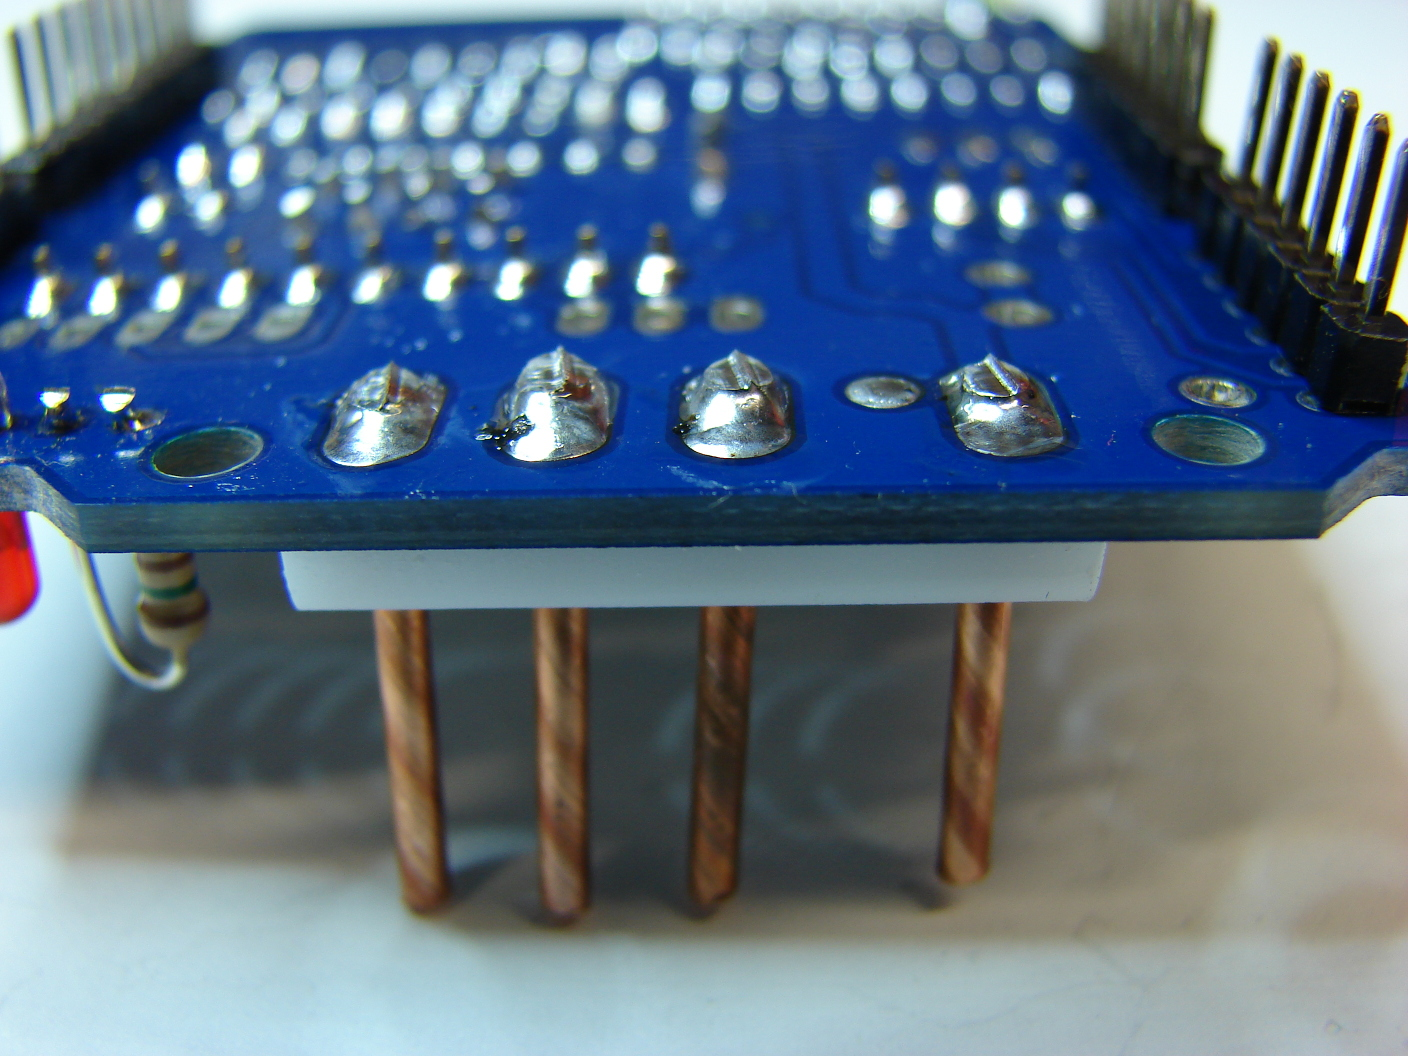
\includegraphics[width=\linewidth]{abb8_2b}
\caption{Avoid short-circuits}
\label{fig:abb8_2b}
\end{figure}

\FloatBarrier

\textbf{KH-900 / KH-965:} \\

KH-900 and KH-965 are not officially supported, yet.
%Verlöten Sie den Hohlstecker entsprechen Abbildung \ref{fig:abb8_3}. \textbf{ACHTUNG!} Die verwendete Polarität trägt den Pluspol an der Außenseite und den Minuspol im Innenleiter. Dies ist die Polarität der original Brother-Netzteile. Bei verwendung von anderen Netzteilen unbedingt auf die richtige Polung achten. Ansonsten kann dies zu Zerstörung von Bauteilen oder gar der Strickmaschine führen.

%\begin{figure}[tbhp]\centering
%
\includegraphics[width=\linewidth]{no}
%\caption{Versorgungsstecker KH-900/965}
%\label{fig:abb8_3}
%\end{figure}

%\FloatBarrier

\subsection*{Last step}

Please double check the orientation and polarity of all parts. Check for short-circuits and the quality of the soldering joints. Check if all projecting wires on the bottom side of the board have been cut off to avoid short-circuits with the Arduino.

%------------------------------------------------

\section{Test and initial operation}

\subsection*{Checklist}

\begin{itemize}[noitemsep] % [noitemsep] removes whitespace between the items for a compact look
\item[\CheckedBox] All parts (especially the ICs and the connectors) have the right orientation.
\item[\CheckedBox] No remains of solder on the shield or any pin of a part.
\item[\CheckedBox] No remains of wire on the shield.
\item[\CheckedBox] No short-circuits visible.
\item[\CheckedBox] Soldering joints look proper.
\end{itemize}

If all of these points are ok, you can put the shield into the Arduino and connect the Arduino to the USB port of a computer. Now, the red LED on the shield should light up.

If no, it is likely that there is a short-circuit or a broken soldering joint - please double check your soldering.

If yes, you can start with the installation of the shield according to the videos on

\url{http://ayab-knitting.com}.

\subsection*{Errors}

If it is likely that a safe operation of the device is not longer possible, the device has to be put out of operation and be saved against unintentional operation.

This is the case when:

\begin{itemize}[noitemsep] % [noitemsep] removes whitespace between the items for a compact look
\item The device has visible damage.
\item The device is not functional any longer.
\item Any part of the device is loose.
\item Wiring is obviously damaged.
\end{itemize}

If the device has to be repaired, you shall only use original spare parts. Usage of third party spare parts may lead to serious physical injury!

The device may only be repaired by an expert!

%------------------------------------------------

\section{Warranty/Disclaimer}

As we do not have any influence on the correct and appropriate installation of this kit, we only can ensure the completeness and quality of the supplied parts.

%Garantiert wird eine den Kennwerten entsprechende Funktion der Bauelemente im uneingebautem Zustand und die Einhaltung der technischen Daten der Schaltung bei entsprechend der Lötvorschrift, fachgerechter Verarbeitung und vorgeschriebener Inbetriebnahme und Betriebsweise.

Any further claims are excluded.

We do not take any liability for damage or secondary damage related to this product.

%Wir behalten uns eine Reparatur, Nachbesserung, Ersatzteillieferung oder Rückerstattung des Kaufpreises vor.

We do not have any liability in case of:

\begin{itemize}[noitemsep] % [noitemsep] removes whitespace between the items for a compact look
\item acid based solder, flux, etc. was used for soldering.
\item the kit was not soldered correctly.
\item modifications of the device or attempted repair of the device.
\item custom modification of the shield.
\item attaching, removing or extending any parts on the shield.
\item usage of any parts which where not part of the kit.
\item destruction of any circuit path or solder pad.
\item wrong assembly/placement of parts.
\item overloading the circuit.
\item damages caused by third party.
\item damages caused by inobservance of the manual and the assembly plan.
\item connection to a wrong voltage or wrong polarity.
\item misusage or damage through careless usage or misusage.
\item defects caused by usage of wrong fuses or overriden fuses.
\end{itemize}

Kits which have been started to be built up or are already built up are nonreturnable.

When working with products which are powered by electrical energy, you shall follow the electrical safety regulations which are  applicable for your country!

%------------------------------------------------

\section{Appendix}

\subsection*{Bill of Materials}

\subsubsection*{Basic Shield}

The basic shield contains all parts which are not related to specific machine models.

 \begin{tabular}{lll}
 \hline
 \textbf{Name}      & \textbf{Type}        & \textbf{Value}  \\ \hline
 PCB                & -                   & -              \\ \hline
 R1/R2              & Resistor 5\%        & 10k\textOmega  \\ \hline
 R3/R4/R5           & Resistor 5\%        & 150\textOmega  \\ \hline
 LED1               & LED wired           & red            \\ \hline
 LED2               & LED wired           & yellow         \\ \hline
 LED2               & LED wired           & green          \\ \hline
 IC1/IC2            & Darlington Array    & ULN2803        \\ \hline
 IC3/IC4            & Darlington Array    & ULN2803        \\ \hline
 JP6                & Molex               & 2-Pin          \\ \hline
 JP9                & 2.54mm Pin Header   & 4-Pin          \\ \hline
 Beeper             & Piezo Beeper        & 4-8V           \\ \hline
 Arduino-Connector  & 2.54mm Pin Header   & -              \\ \hline
 \end{tabular}\\

 \subsubsection*{Connectors KH-910/KH-930}

\begin{tabular}{lll}
\hline
\textbf{Name}      & \textbf{Type}       & \textbf{Value}  \\ \hline
JP1                & Power connector     & proprietary  \\ \hline
JP2                & 2.5mm Pin Header    & 3-Pin        \\ \hline
JP3                & 2.5mm Pin Header    & 8-Pin        \\ \hline
JP4/JP5            & 2.5mm Pin Header    & 10-Pin       \\ \hline
Extension cable    & 30cm ribbon cable   & 3-Pin        \\ \hline
\end{tabular}\\

\subsubsection*{Connectors KH-930}

\begin{tabular}{lll}
\hline
\textbf{Name}      & \textbf{Type}        & \textbf{Value}  \\ \hline
JP1                & Power connector     & proprietary    \\ \hline
JP2/JP7            & 2.5mm Molex         & 3-Pin        \\ \hline
JP3                & 2.5mm Molex         & 8-Pin        \\ \hline
JP4                & 2.5mm Molex         & 10-Pin       \\ \hline
JP8                & 2.5mm Molex         & 5-Pin        \\ \hline
Extension cable    & 30cm ribbon cable   & 3-Pin        \\ \hline
\end{tabular}\\

 \begin{figure}[tbhp]\centering
 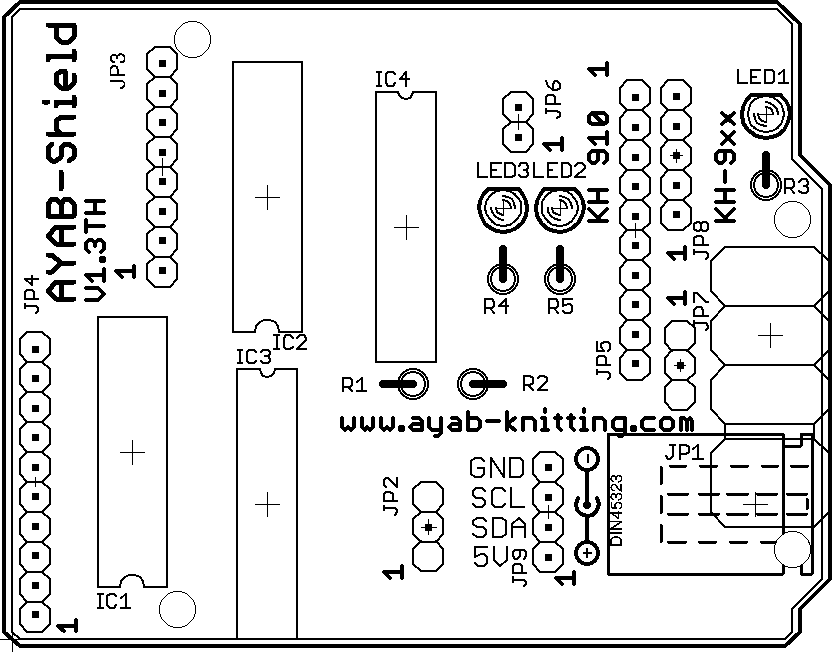
\includegraphics[width=\linewidth]{shield}
 \caption{Layout diagram}
 \end{figure}

 \FloatBarrier

 \begin{figure*}[tbhp]\centering % Using \begin{figure*} makes the figure take up the entire width of the page
 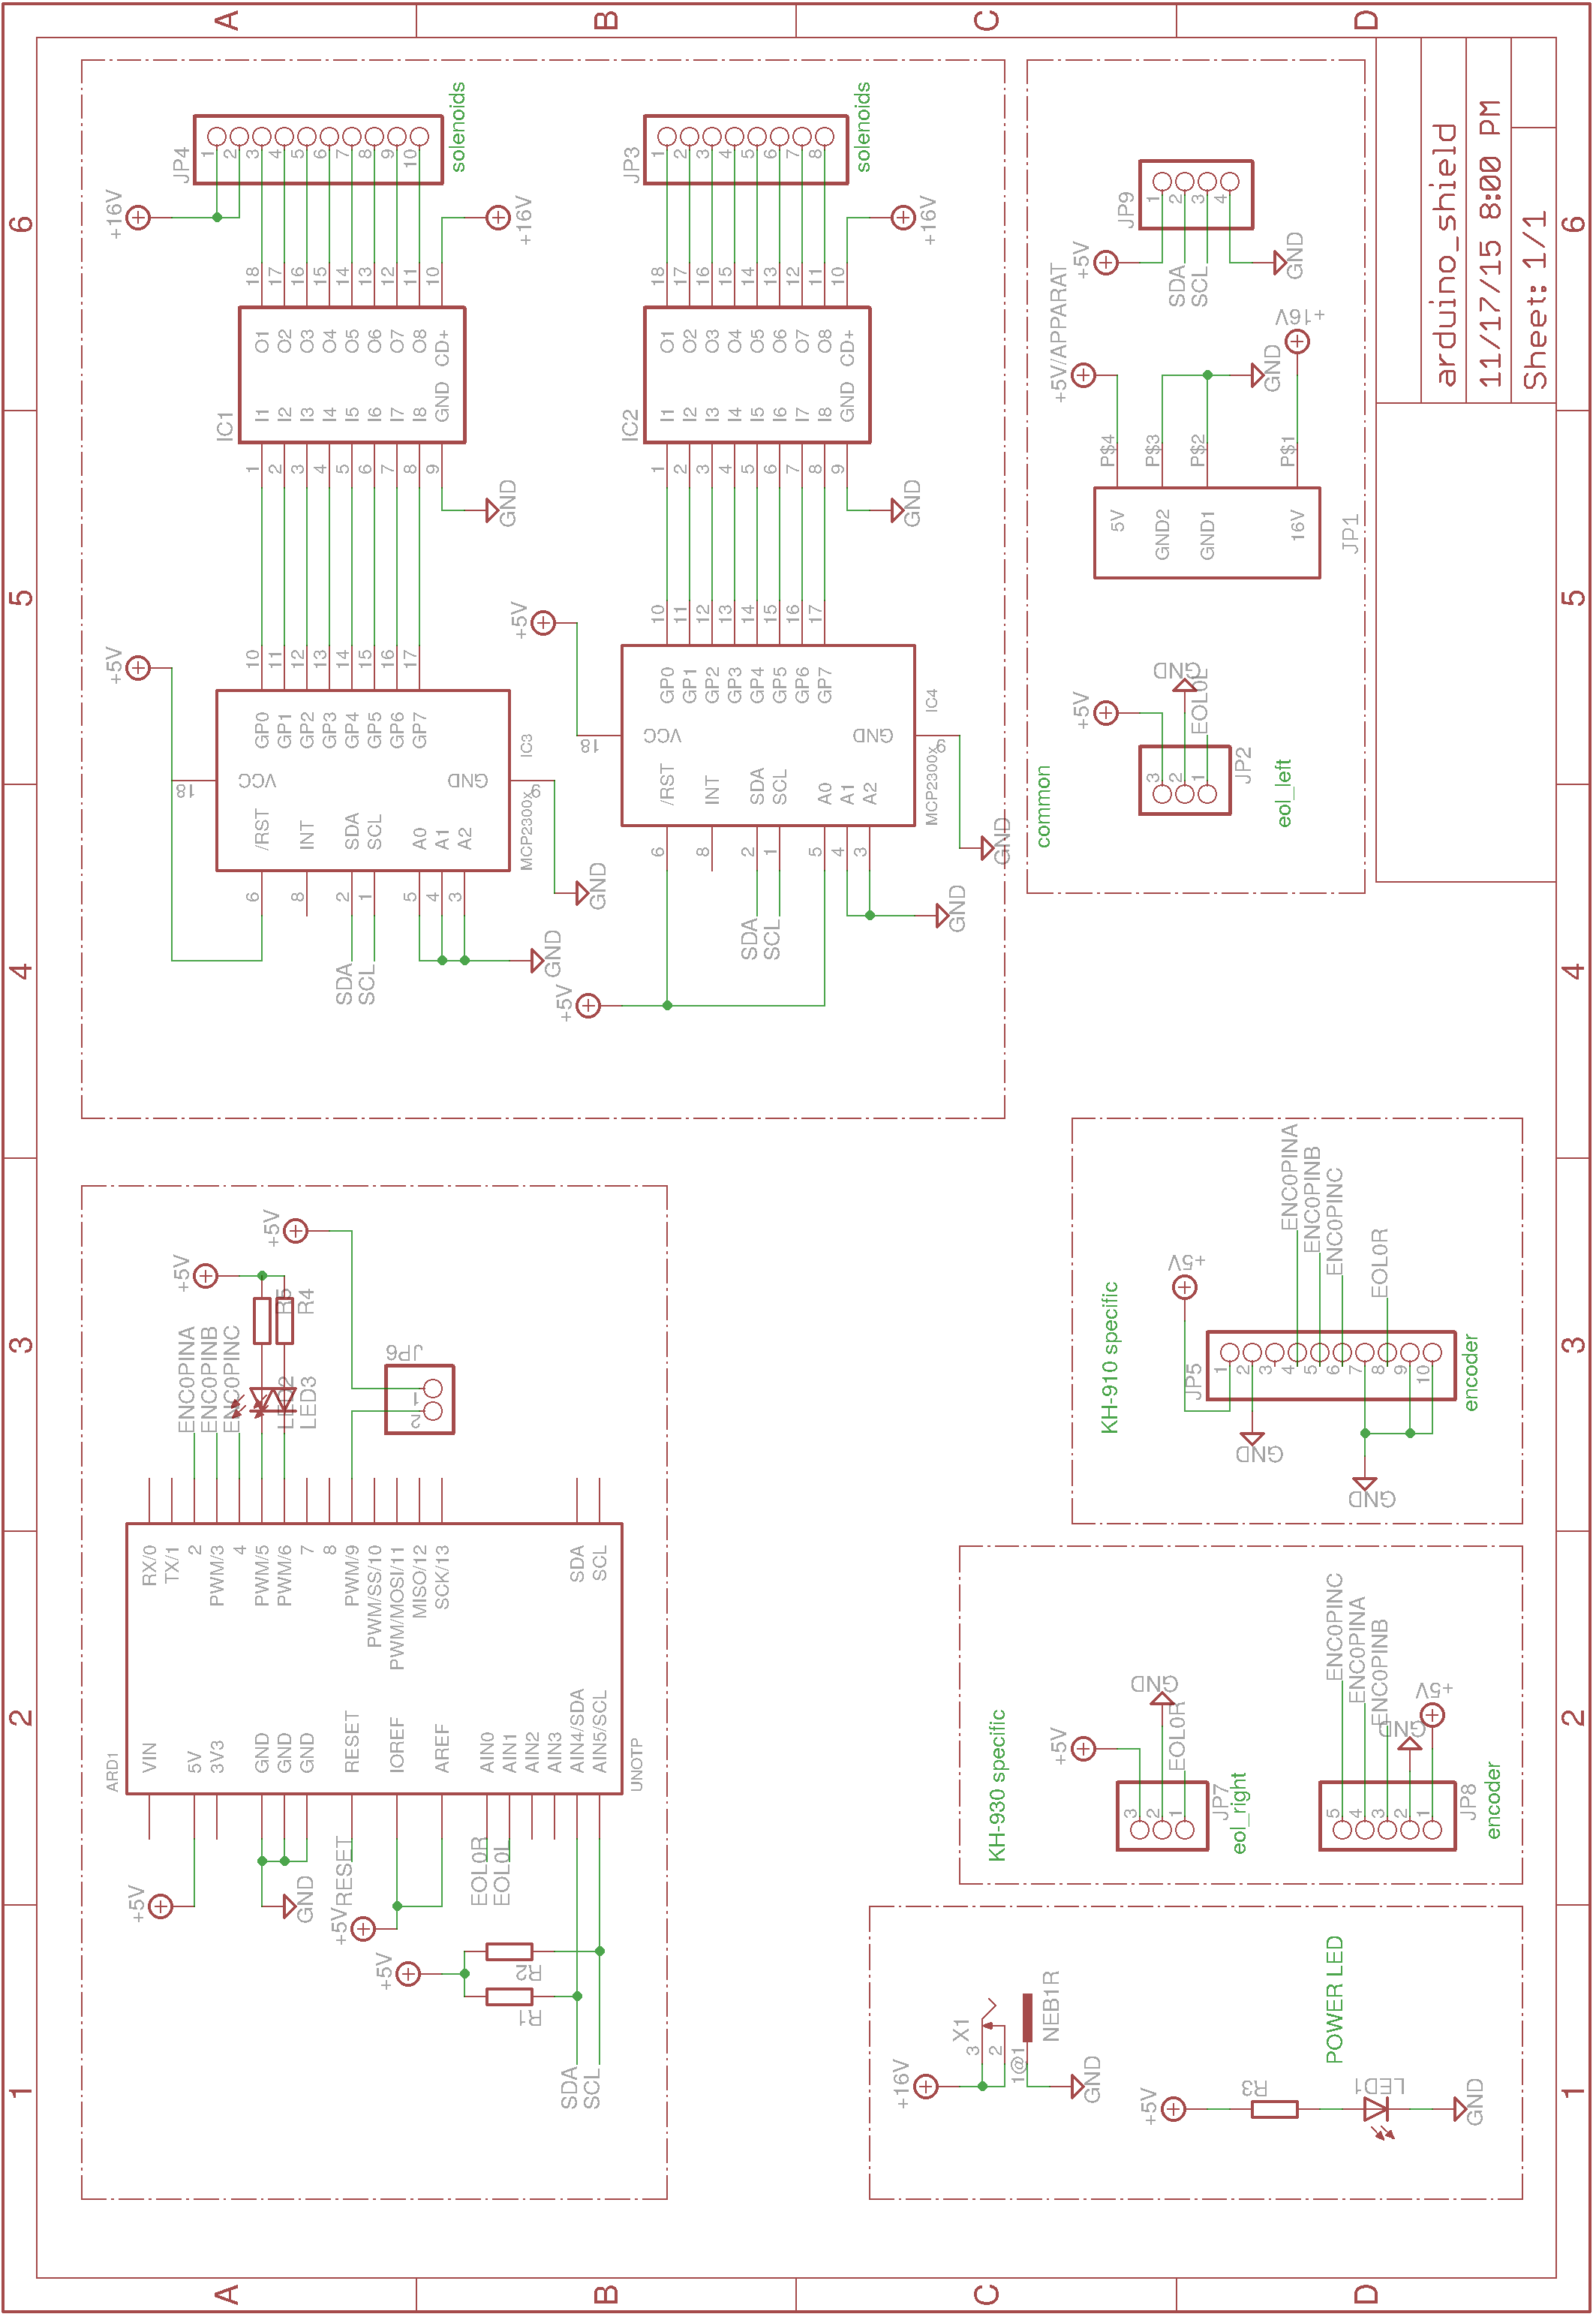
\includegraphics[width=0.9\linewidth]{schaltplan}
 \caption{Schematic diagram}
 \end{figure*}

\FloatBarrier
%------------------------------------------------

\phantomsection
\section*{Imprint} % The \section*{} command stops section numbering

\addcontentsline{toc}{section}{Imprint} % Adds this section to the table of contents

\begin{figure}[tbhp]

\includegraphics[width=0.3\linewidth]{cc}
\end{figure}

\textbf{Address:}

thinkstack UG

Tuerkenstrasse 21

80799 Muenchen

\url{http://thinkstack.de}

%----------------------------------------------------------------------------------------
%   REFERENCE LIST
%----------------------------------------------------------------------------------------
\phantomsection
\bibliographystyle{unsrt}
%\bibliography{sample}

%----------------------------------------------------------------------------------------

\end{document}